%%% Lecture 8

\lecture[We actually prove the story about the long exact sequence associated to a fibre bundle.]{2021-11-10}

Before we get to the promised results, we prove an auxiliary one.\rightnote{\Attention\ Didn't sleep much the night before this one, I hope I didn't type anything too stupid!}

\begin{lemma}\label{lemma:equivalent-HCP}
Let $p:E\to B$ be a map. The following are equivalent:
\begin{numerate}
\item $p$ is a Serre fibration,
\item $p$ has the absolute HLP for $D^n$ for all $n$,
\item $p$ has the relative HLP for $(D^n,\de D^n)$ for all $n$,
\item $p$ has the relative HLP for all relative CW-complexes.
\end{numerate}
\end{lemma}

\begin{proof}

$(1)\implies(2)$ This is true because $D^n$ is a CW-complex.

$(2)\implies(3)$ The space pairs $(D^n\times[0,1],D^n\times\cb{0})$ and $(D^n\times[0,1],D^n\times\cb{0}\cup\de D^n\times[0,1])$ are homeomorphic, hence any test situation for one HLP can be translated into a test situation for the other, and similarly for the solutions.

$(3)\implies(4)$ Let $(X,X')$ be a relative CW-complex. Consider the test situation:
\begin{center}
    \begin{tikzcd}
    X\times\cb{0}\cup X'\times[0,1] \arrow[d] \arrow[r,"f"] & E \arrow[d,"p"] \\
    X\times[0,1] \arrow[r] & B
    \end{tikzcd}
\end{center}

We first assume that $X=X'\cup_{\de D^n}D^n$ is obtained from $X'$ by attaching a single cell, with characteristic map $\alpha:D^n\to X$.

We obtain:

\begin{center}
    \begin{tikzcd}[row sep=huge]
    D^n\times\cb{0} \cup\de D^n\times[0,1] \arrow[d] \arrow[r] & X\times\cb{0} \cup X'\times[0,1] \arrow[d] \arrow[r,"f"] & E \arrow[d,"P"] \\
    D^n\times[0,1] \arrow[urr,dashed,crossing over,shift right,"H'"] \arrow[r,swap,"\alpha\times\id_{[0,1]}"] & X\times[0,1] \arrow[r,swap,"H"] & B
    \end{tikzcd}
\end{center}

By assumption, there exists a lift $H'$ as in the diagram.

Then the desired solution is
\[X\times[0,1]=(X'\times[0,1])\cup_{\de D^n\times[0,1]}D^n\times[0,1]\xto{f\cup H'}E.\]

The case where $(X,X')$ has finitely many relative cells follows by induction, the infinite case by passing to the colimit.

$(4)\implies(1)$ This is the special case $(X,\emptyset)$.
\end{proof}

\begin{remark}
CW-complexes are colimits of their skeleta.

\begin{center}
    \begin{tikzcd}
    \sk_n X\times[0,1] \arrow[r] \arrow[d,hook] & E \\
    \sk_{n+1}X\times[0,1] \arrow[ur,]
    \end{tikzcd}
\end{center}

We have
\[X\cong\colim_n\sk_n X\]
and since\rightnote{This is the first instance of the fact (which we will use very often) that \href{http://nlab-pages.s3.us-east-2.amazonaws.com/nlab/show/adjoints+preserve+(co-)limits}{adjoints preserve (co-)limits}.} the results in theorem \ref{theorem:exponential-law} assure us that the endofunctor $-\times Z$ of $\Top$ is a left adjoint (to the \enquote{exponentiation} functor; this is AT1Sheet11.2), we have
\[X\times[0,1]\cong\colim_n(\sk_n X\times[0,1]).\]
\end{remark}

Now we can prove the results promised at the end of last lecture.

\begin{lemma}
Let $p:E\to B$ be a Serre fibration, $Y\subset B$ and $x\in p^{-1}(Y)$. Then $p$ induces an isomorphism
\[p_*:\pi_n(E,p^{-1}(Y),x)\xto{\cong}\pi_n(B,Y,p(x))\]
for all $n\geq1$.
\end{lemma}

\begin{proof}
Surjectivity. Let $[\beta]\in\pi_n(B,Y,p(x))$ be represented by $\beta:(I^n,\de I^n,s_0)\to(B,Y,p(x))$ with $s_0=(0,\dots,0)$.
\begin{center}
    \(
    \begin{tikzcd}
    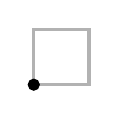
\begin{tikzpicture}[x=2em, y=2em, baseline=0.7em]
        \draw[very thick, black!30] (0,0)--(1,0)--(1,1)--(0,1)--(0,0);
        \filldraw (0,0) circle (2pt);
    \end{tikzpicture}
    \ar[r, hook]\ar[d]
    & 
    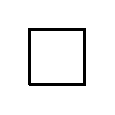
\begin{tikzpicture}[x=2em, y=2em, baseline=0.7em]
        \draw[very thick] (0,0)--(1,0)--(1,1)--(0,1)--(0,0);
    \end{tikzpicture} 
    \ar[r, hook]\ar[d]
    &
    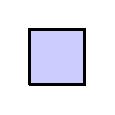
\begin{tikzpicture}[x=2em, y=2em, baseline=0.7em]
        \filldraw[very thick, fill=blue!20] (0,0)--(1,0)--(1,1)--(0,1)--(0,0);
    \end{tikzpicture}
    \ar[d]\\
    p(x)\ar[r, hook]&Y\ar[r, hook]&B
    \end{tikzcd}
    \)
\end{center}

To find a map $(I^n,\de I^n,s_0)\to(E,p^\inv(Y),x)$ mapped to $\beta$ by $p_*$, we would want to lift a homotopy of $\beta|_{I^\ni\times\cb{0}}$, as $\beta$ already looks like one. However, we cannot do this right away, because we are missing a lift of $\beta|_{I^\ni\times\cb{0}}$ to $E$. An obvious way to go about this is by repeated applications of the HLP, but since we are working with a contractible space, there is an easier and faster way.

Applying the HEP first to the relative CW-complex $(\de I^n,I^\ni\times\cb{0})$ for maps to $Y$, second for the relative CW-complex $\pair$ for maps to $B$, we can replace $\beta$ by an homotopic map $\beta'$ which sends all of $I^\ni\times\cb{0}$ to $p(x)$.

\input{Pictures/Lec8Pic2}

Now, the constant map $c_{p(x)}:I^\ni\times\cb{0}\to Y$ can be lifted to E via the constant map $c_x:I^\ni\times\cb{0}\to p^{-1}(Y)$, hence we have a test situation:
\begin{center}
    \begin{tikzcd}[column sep=large]
    I^\ni\times\cb{0} \arrow[d] \arrow[r,"c_x"] & E \arrow[d,"p"] \\
    I^n \arrow[r,swap,"\beta'"] \arrow[ur,dashed,"\exists\til\beta"] & B
    \end{tikzcd}
\end{center}
Since $p$ is a Serre fibration, there exists $\til\beta:I^n\to E$ such that $\til\beta|_{I^\ni\times\cb{0}}=c_x$, so that $\til\beta(s_0)=x$, and $p\circ\til\beta=\beta'$, so that $\til\beta(\de I^n)\subset p^{-1}(Y)$. Hence $\til\beta$ represents an element $[\til\beta]$ of $\pi_n(E,p^{-1}(Y),x)$, which by construction maps to $[\beta']=[\beta]$ under $p_*$.

Injectivity. Let $\alpha_1,\alpha_2:(I^n,\de I^n,s_0)\to(E,p^{-1}(Y),x)$ represent elements of $\pi_n(E,p^{-1}(Y),x)$ which are sent to the same element under $p_*$. Then there exists a homotopy of triple maps $H:I^n\times I\to B$ from $p\circ\alpha_1$ to $p\circ\alpha_2$.

\[
\begin{tikzcd}[column sep = huge]
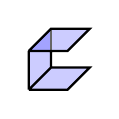
\begin{tikzpicture}[x = 1.4em, y = 1.4em, z = 0.8em, baseline = 0.4em]
    \begin{scope}[fill=blue, opacity=0.2]
    \fill
    (0,0,0) -- (0,1,0) -- (0,1,1) -- (0,0,1) -- (0,0,0);
    \fill
    (0,0,0) -- (1,0,0) -- (1,0,1) -- (0,0,1) -- (0,0,0);
    \fill
    (0,1,0) -- (1,1,0) -- (1,1,1) -- (0,1,1) -- (0,1,0);
    \end{scope}
    \begin{scope}[thick]
    \draw[black!60]
    (0,0.4,1) -- (0,1,1);
    \draw
    (0,0,1) -- (0,0.45,1)
    (0,0,0) -- (0,1,0)
    (0,0,0) -- (1,0,0) -- (1,0,1) -- (0,0,1) -- (0,0,0)
    (0,1,0) -- (1,1,0) -- (1,1,1) -- (0,1,1) -- (0,1,0);
    \end{scope}
\end{tikzpicture}
\ar[r, "\alpha_1\cup c_x\cup\alpha_2"] \ar[d] & E \ar[d, " p"]\\
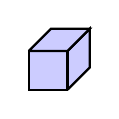
\begin{tikzpicture}[x = 1.4em, y = 1.4em, z = 0.8em, baseline = 0.4em]
    \begin{scope}[fill=blue!20, thick]
    \filldraw
    (1,0,0) -- (1,1,0) -- (1,1,1) -- (1,0,1) -- (1,0,0);
    \filldraw
    (1,0,0) -- (1,1,0) -- (0,1,0) -- (0,0,0) -- (1,0,0);
    \filldraw
    (0,1,0) -- (1,1,0) -- (1,1,1) -- (0,1,1) -- (0,1,0);
    \end{scope}
\end{tikzpicture}
\ar[r, "H"'] \ar[ur, dashed] & B
\end{tikzcd}\rightnote{Note that for this to work we have to \enquote{swap} the last two coordinates!}
\]

Again we can assume that $\alpha_1(I^\ni\times\cb{0})=\alpha_2(I^\ni\times\cb{0})=\cb{x}$. In addition we can assume that $H$ sends $(I^\ni\times\cb{0})\times I$ constantly to $p(x)$. We again lift $c_{p(x)}$ to $c_x$ and view $\alpha_1$ and $\alpha_2$ as lifts of $H$ on the subspace $I^\ni\times\cb{0}\times\cb{0}\cup I^\ni\times\cb{0}\times\cb{1}$. Since $(I^\ni\times\cb{0}\times I,I^\ni\times\cb{0}\times\cb{0}\cup I^\ni\times\cb{0}\times\cb{1})$ is a relative CW-complex, we can apply the relative HLP to lift $H$ to a map $\til H:I^n\times I\to E$, giving a relative homotopy from $\alpha_1$ to $\alpha_2$.
\end{proof}

We remember that this has as a consequence the long exact sequence associated to a Serre fibration.

\begin{theorem}
Let $Y=\cb{b}$, $F=p^{-1}(b)$. We get a long exact sequence:
\[\cdots\to\pi_n(F,x)\to\pi_n(E,x)\to\pi_n(E,F,x)\cong\pi_n(B,b)\to\cdots\]
\end{theorem}

Many examples of Serre fibrations come from fibre bundles, thanks to the next theorem.

\begin{theorem}
Every fibre bundle is a Serre fibration.
\end{theorem}

\begin{proof}
Let $p:E\to B$ be a fibre bundle and a lifting problem
\begin{center}
    \begin{tikzcd}
    X\times\cb{0} \arrow[r,"f"] \arrow[d] & E \arrow[d,"p"] \\
    X\times I \arrow[r,"H"] & B
    \end{tikzcd}
\end{center}

Easy case. Let $p$ be globally trivial, i.e. of the form $\pr_B:B\times F\to B$ for some space $F$. Then we have
\begin{center}
    \begin{tikzcd}[column sep=large]
    X\times\cb{0} \arrow[r,"{(f_1, f_2)}"] \arrow[d] & B\times F \arrow[d,"\pr_B"] \\
    X\times I \arrow[r,swap,"H"] \arrow[ur,dashed,"\til H"] & B
    \end{tikzcd}
\end{center}
We can define a lift $\til H$ explicitly via $\til H(x,t)=(H(x,t),f_2(x))$ (this works for any space $X$).

General case. We have to glue local lifts together systematically.

By lemma \ref{lemma:equivalent-HCP}, it suffices to check the HLP for disks $D^n$, or equivalently for cubes $I^n$. Hence we are given:
\begin{center}
    \begin{tikzcd}
    I^n\times\cb{0} \arrow[r,"f"] \arrow[d] & E \arrow[d,"p"] \\
    I^n\times I \arrow[r,"H"] & B
    \end{tikzcd}
\end{center}

Let $\cb{U_i}_{i\in I}$ be an open covering of $B$, such that $p^{-1}(U_i)\xto{p}U_i$ is a trivial fibre bundle for all $i$. Pulling back along $H$, we get an open cover of $I^n\times I$. By Lebesgue's lemma, we can divide $I^n\times I$ into smaller cubes of side length $1/k$, such that each cube is contained in some $p^{-1}(U_i)$.\rightnote{The drawing is an explanation of how \enquote{row by row}               is fine and otherwise not: this is because the HLP lets us lift the \enquote{base} of the little cubes (or some more, in the relative case), but in the situation pictured on the right there is no way to be sure that our lifting will coincide with the map we already have in the upper side of the cube.}
\input{Pictures/Lec8Pic3}\medskip

We can then extend $H$ iteratively over the smaller cubes \enquote{row by row}. In every situation this amounts to choosing a solution to the relative lifting problem for a globally trivial fibre bundle.
\end{proof}

\begin{remark}
Not every fibre bundle is a Hurewicz fibration (but actual counter-examples are complicated). A sufficient condition is that the base space be paracompact.
\end{remark}

\begin{remark}

An interesting question: are liftings of homotopies unique? It turns out that they are unique up to homotopy! Indeed, let $\til H_1$ and $\til H_2$ two liftings of an homotopy $H$, then we can apply the HLP to obtain a homotopy between them: 
\begin{center}
    \begin{tikzcd}[column sep=huge]
    X\times\cb{0} \arrow[r] \arrow[d] & E \arrow[d,"p"] \\
    X\times I \arrow[r,"H"'] \arrow[ur,dashed,"\til H_1", "\til H_2"'] & B
    \end{tikzcd}\qquad
    \begin{tikzcd}[column sep=huge]
    X\times I\times\cb{0} \cup X\times I\times\cb{1} \arrow[r,"\til H_1\cup\til H_2"] \arrow[d] & E \arrow[d,"p"] \\
    X\times I\times I \ar[ur,dashed,shift right=1] \arrow[r,"\const_H"'] & B
    \end{tikzcd}
\end{center}\normalmarginpar
\end{remark}
